\documentclass[a4paper,12pt]{article}
%\usepackage{verbatim}


\usepackage{amssymb}
\usepackage{amsmath}
\usepackage{amsthm}
\usepackage{tikz}
\usepackage{enumerate}
\usepackage{mathrsfs}
\usepackage{graphicx}
\usepackage{cite}

\usetikzlibrary{arrows,snakes,backgrounds,positioning,shadows}

\tikzstyle{stan} = [circle,draw=red!50,fill=red!20,thin]

\begin{document}

\title{Control Optimization of Water System for Aeroponics}
\author{Oliver Hennigh \\
Clarkson University}
\renewcommand{\today}{}

\maketitle

\newtheorem*{t1}{Theorem}
\newtheorem*{t3}{Lemma}
\newtheorem*{t2}{Definition}

\begin{abstract}
		  We have created a model to mimic the behavior of aeroponic water system. Using search algorithms we found optimal or sub optimal control scheme for such systems. The aeroponic water system of investigation uses air compressor to spray fine mists onto free roots of various plants \cite{schorr1985method}. Optimization occurs for both correct moisture percent in roots and compressor active time. We propose our model be used to optimize Clarkson Universities Greenhouse project.
\end{abstract}


\section{Introduction}

In aeroponics nutrient rich water is sprayed onto the free hanging root system of plants. This method of cultivation has many benefits including maximal oxygen intake and high nutrient uptake. The main drawback is the method's need for mist production. It is common that compressors are used to store air pressure and release mists at periodic intervals \cite{schorr1985method}. This system is used by Clarkson Universities Greenhouse project and has prompted our interest in modeling it. 

The model consist of a compressor, pressure tank, mist pipe and root system. The compressor is activated when the pressure tank drops to a threshold pressure. This causes the compressor to be activated for a pre-calculated amount of time. The mist pipe switches on and off at a particular frequency and period. The root system is modeled as a drying system with a given max moisture content and linear evaporation rate. Normaly drying systems are modeled as complicated negative exponentials \cite{amer2003new} \cite{mujumdar2000fundamental}.

\subsection{Mathematics of Model}
Several assumptions are made about each aspect of the model. There is an assumed linear drying rate of the roots. The mist spray rate is linear dependent on the pressure of the tank. The compressor is assumed to increase pressure at a constant rate. Modeling this with equations we get the system


\begin{table}[ht]
\caption{Constants of Interest}
\centering
\begin{tabular} {c c}
\hline\hline
 Variable & explanation \\ [0.5ex]
\hline
$P_m$ & air loss rate from mister \\
$W_m$ & water spray rate from mister \\
$E_r$ & evaporation rate of roots \\ 
$M_m$ & max moister content of roots \\ 
$V_t$ & volume of tank \\
$C_r$ & compression rate of compressor \\
$M_c(t)$ & mist control function with values 0 or 1 \\
$P_c(t)$ & pump control function with values 0 or 1 \\
$M(t)$ & moister content of roots in percent \\
$V(t)$ & volume of air compressed in tank \\
\hline
\end{tabular}
\end{table}

\begin{equation}
		  V(t+1) = V(t) + C_r P_c(t) - P_m \frac{V(t)}{V_t} M_c(t)
\end{equation}

\begin{equation}
		  M(t+1) = M(t) + W_m \frac{V(t)}{V_t} M_c(t) - E_r
\end{equation}

\subsection{Optimization}

We wish to optimize both the power usage of the compressor as well as maintaining ideal moister content in the roots. We have included a cost function for the number of times the compressor is activated. This is because starting the compressor often takes several times as much energy as running it. This model was inspired by other optimization problems in greenhouses \cite{chalabi1996real}. Putting this together gives the following optimization problem.

\begin{table}[ht]
\caption{Optimization constants}
\centering
\begin{tabular} {c c}
\hline\hline
 Variable & explanation \\ [0.5ex]
\hline
$I_m$ & Ideal moister content of root \\
$C_s$ & Cost for turning the compressor on \\
$\lambda_r$ & importance factor of root moisture \\
$\lambda_m$ & importance factor of motor usage \\ 
\hline
\end{tabular}
\end{table}

\begin{equation}
		  O = \lambda_r || I_m - M(t) || + \lambda_m || P_c(t) + C_s||
\end{equation}

Because this optimization takes into account both moisture expressions and cost of running the compressor we have included constants $\lambda_r$ and $\lambda_m$ to control the importance of each component.


\subsection{Search Space}

The hope for optimizing these equations was to use calculus of variations however there are several real world constraints that make this difficult. Both the mist and pump control must be discrete 0, 1 for relevance to the Clarkson greenhouse project. I believe that the problem can still be solved analytically however in the interest of time we have coded the model and simply searched for the optimal solution. Our search space is inspired by the system currently used at Clarkson. 

\begin{table}[ht]
\caption{Search Space}
\centering
\begin{tabular} {c c}
\hline\hline
 Variable & explanation \\ [0.5ex]
\hline
$F_m$ & frequency of mister activation \\
$M_t$ & mist activation time \\
$T_p$ & threshold pressure to activate compressor \\ 
$C_t$ & compressor activation time \\ 
\hline
\end{tabular}
\end{table}

By randomly trying combinations of these values and running our model on them we could discover the optimal or sub optimal solutions.

\subsection{Applying to Clarkson's Greenhouse project}

Our proposed model is highly dependent on many unknown constants. These values can be found by performing simple experiments and calculations. To illustrate this we have included several instructions on obtaining various constants. To validate our model we will need to determine these constants on the greenhouse data and record data on plant moister content as well as tank pressure. If our model produces similar data with the appropriate constants then it will validate our results.


\begin{table}[ht]
\caption{Constants cook book}
\centering
\begin{tabular} {p{1 cm} p{9cm}}
\hline\hline
 Variable & method \\ [0.5ex]
\hline
$P_m$ & Measure pressure decrease of tank vs time and do a linear interpolation. Calculated volume change from pressure change \\
$W_m$ & Weight weight increase of root vs time with mist on and do linear interpolation. \cite{varney1993rates} \\
$E_r$ & Weight root system while drying and do linear interpolation. It should follow a negative exponential. \\ 
$M_m$ & Compare weight of soaked root and completely dry root. \\ 
\hline
\end{tabular}
\end{table}


\section{Data and Results}

We have coded our model and run several simulations. The following data is the result of the following realistic constant values.


\begin{table}[ht]
\caption{Test Model}
\centering
\begin{tabular} {c c}
\hline\hline
 Variable & value \\ [0.5ex]
\hline
$P_m$ & .3 units per second\\
$W_m$ & .01 percent per second \\
$E_r$ & .0002 percent per second\\ 
$M_m$ & .16 percent \\ 
$V_t$ & 10 units \\
$C_r$ & 2 units \\
$I_m$ & .08 \\
$C_s$ & 3.0 \\
$\lambda_r$ & 3.0 \\
$\lambda_m$ & 1.0 \\ 
\hline
\end{tabular}
\end{table}

By searching on the space described above we obtained and optimal configuration seen bellow. The time period examined was 24 hours.

\begin{table}[ht]
\caption{Optimal Solution}
\centering
\begin{tabular} {c c}
\hline\hline
 Variable & value \\ [0.5ex]
\hline
$F_m$ & 150 seconds \\
$M_t$ & 5 seconds \\
$T_p$ & 3.69 \\ 
$C_t$ & 2 seconds \\ 
\hline
\end{tabular}
\end{table}

These results are not particularly interesting however they prove that this method works and demonstrates its power.


\section{Produced Data}

If we plot the volume compressed and root moisture content, several interesting aspects can be seen. The root graph shows fairly drastic change from 3 percent to 9 percent water content. It can be seen by zooming in on the graph that there are two levels of oscillation present. One from the repetitive mist control and the other from the change in pressure of the tank. The pressure tank graph shows when the motor is turned off and on. It comes to around 6 times per hour and activates for only 2 seconds at a time. This frequent oscillation between on and off is probably the result of too low a penalty for turning the compressor on and off.

\begin{figure}[ht!]
	\centering
	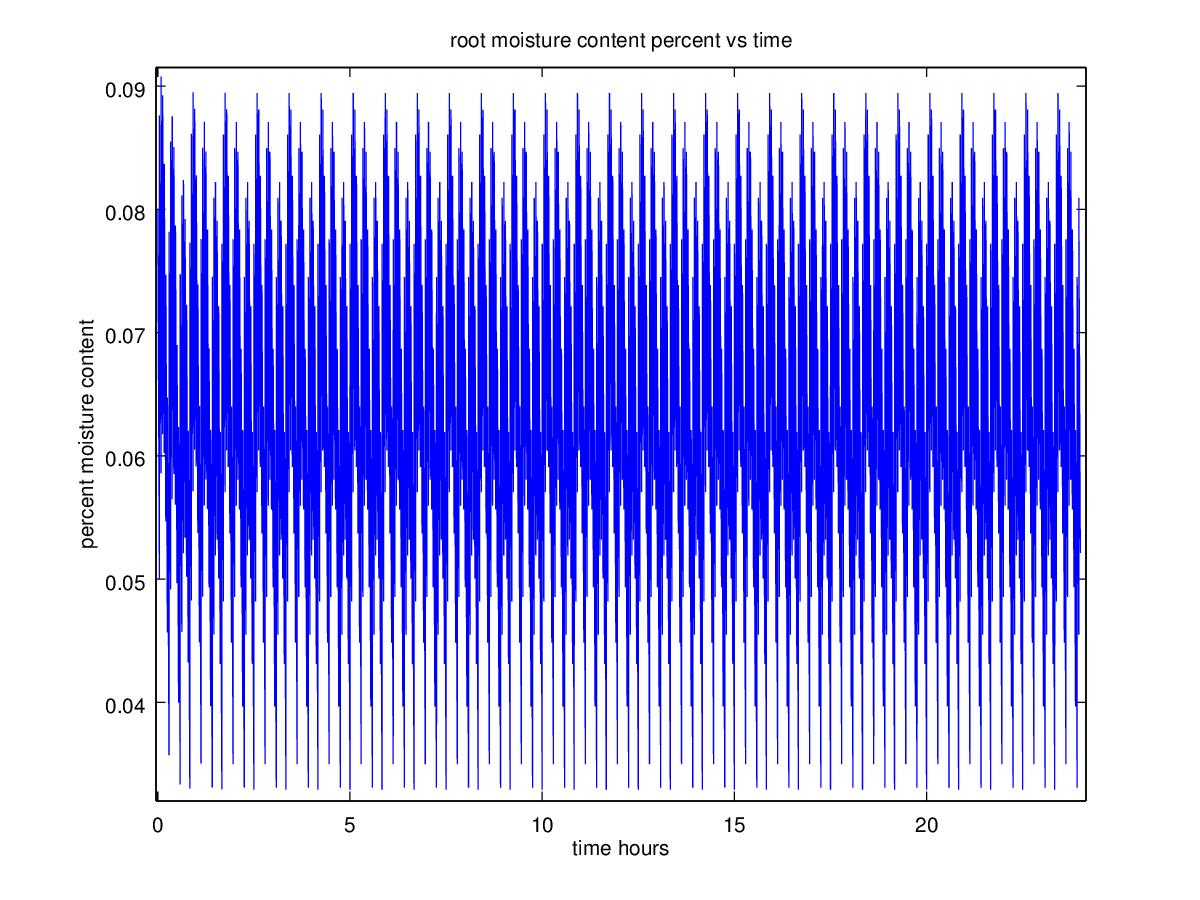
\includegraphics[width=60mm]{root_moisture_content_1.jpg}
	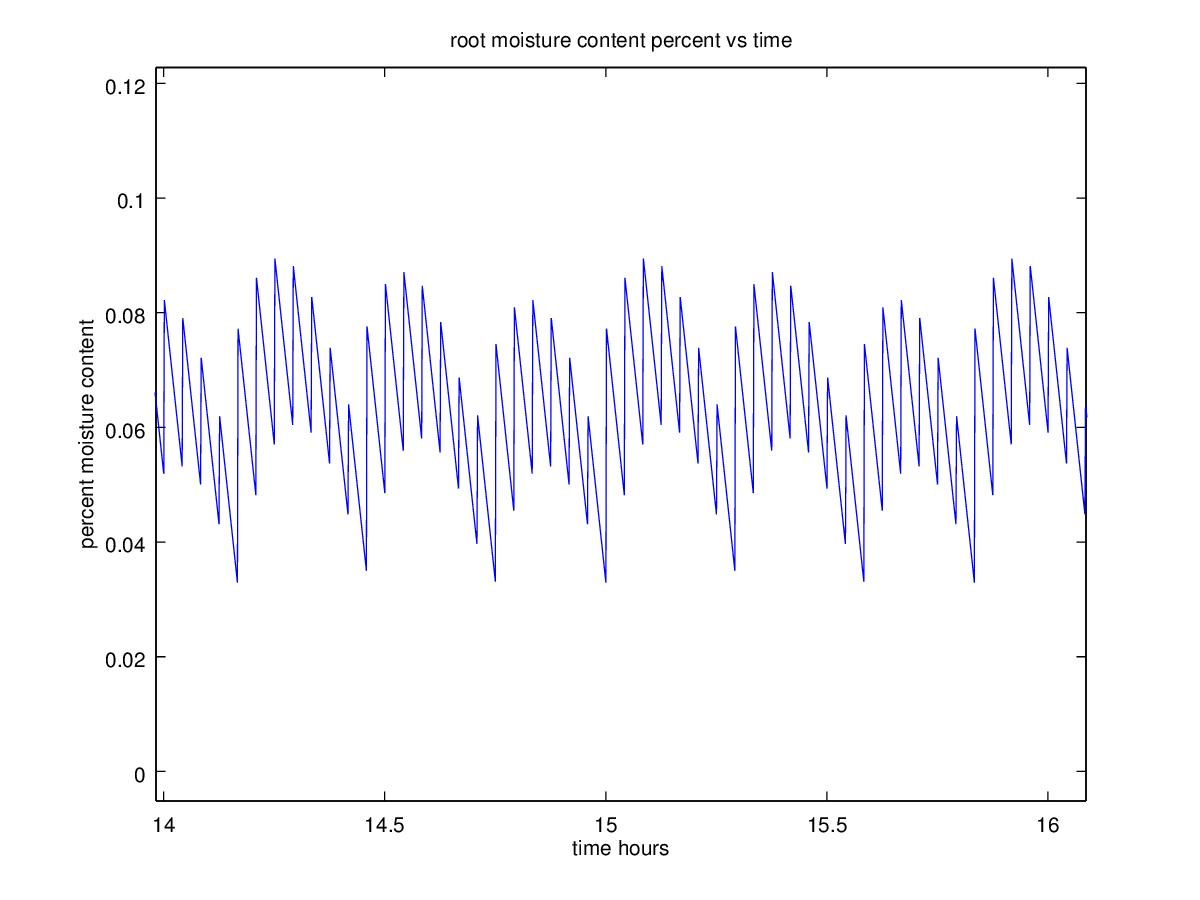
\includegraphics[width=60mm]{root_moisture_content_2.jpg}
	\caption{root moisture content}
\end{figure}

\begin{figure}[ht!]
	\centering
	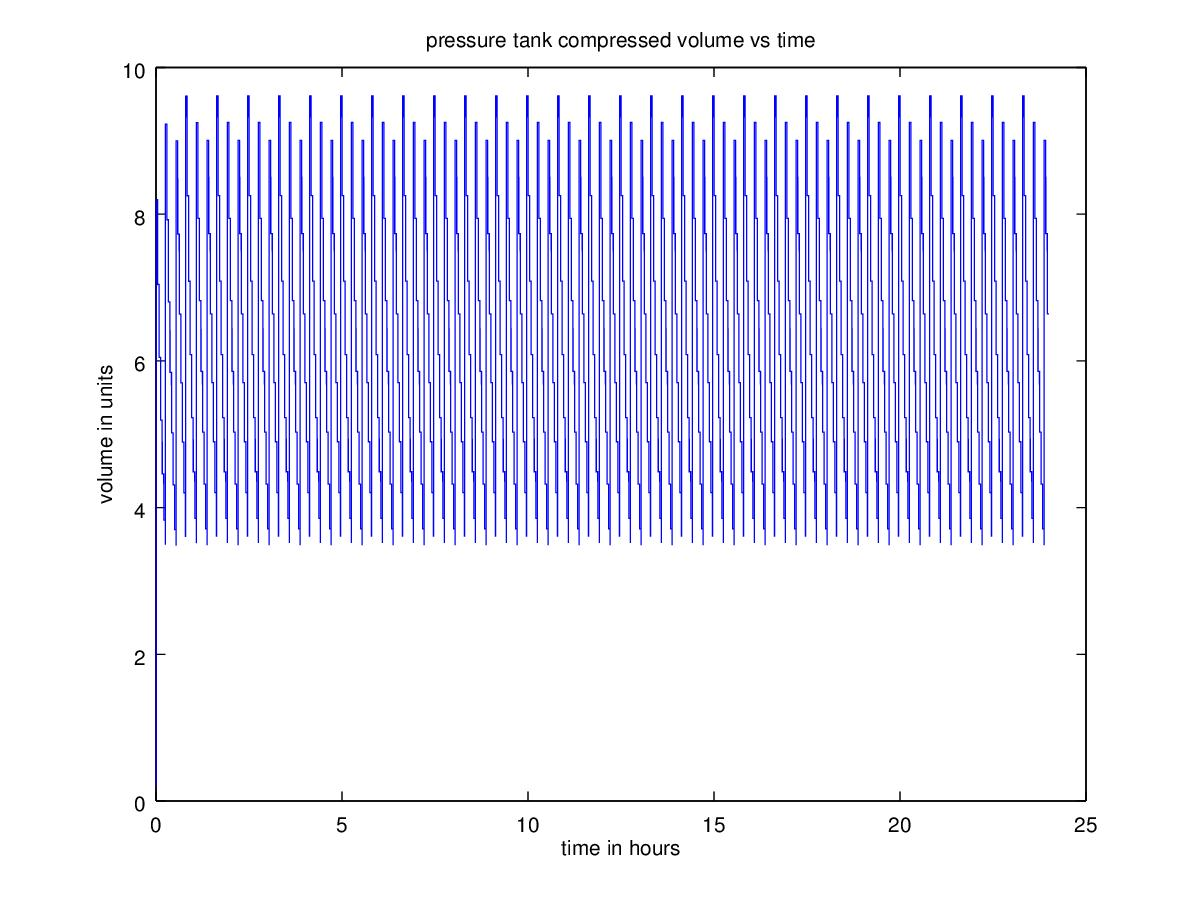
\includegraphics[width=60mm]{pressure_tank_compressed_volume_1.jpg}
	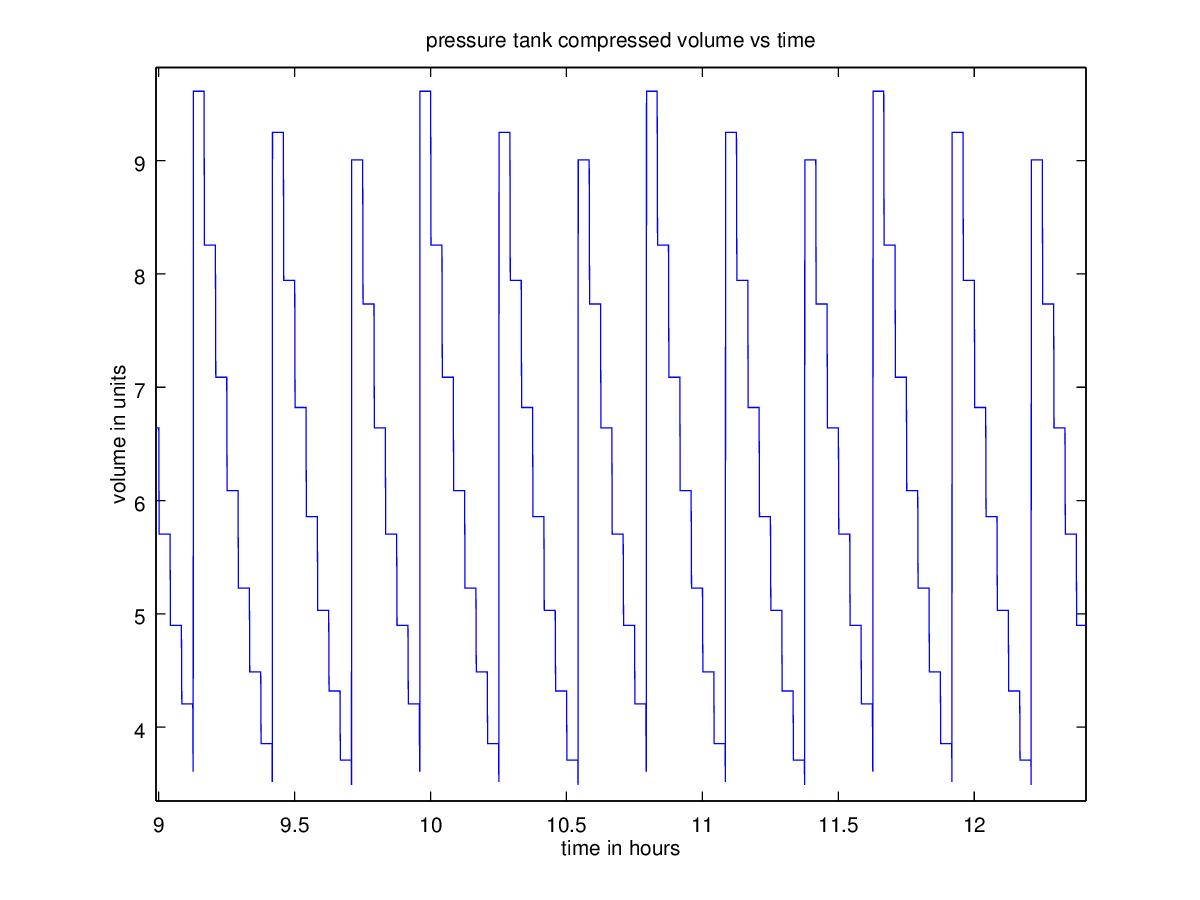
\includegraphics[width=60mm]{pressure_tank_compressed_volume_2.jpg}
	\caption{pressure tank compressed}
\end{figure}

\subsection{Distribution of Optimization Points}

A very interesting effect can be seen if we run this greenhouse simulation many times and plot their fitness value vs number of occurrences.

\begin{figure}[ht!]
	\centering
	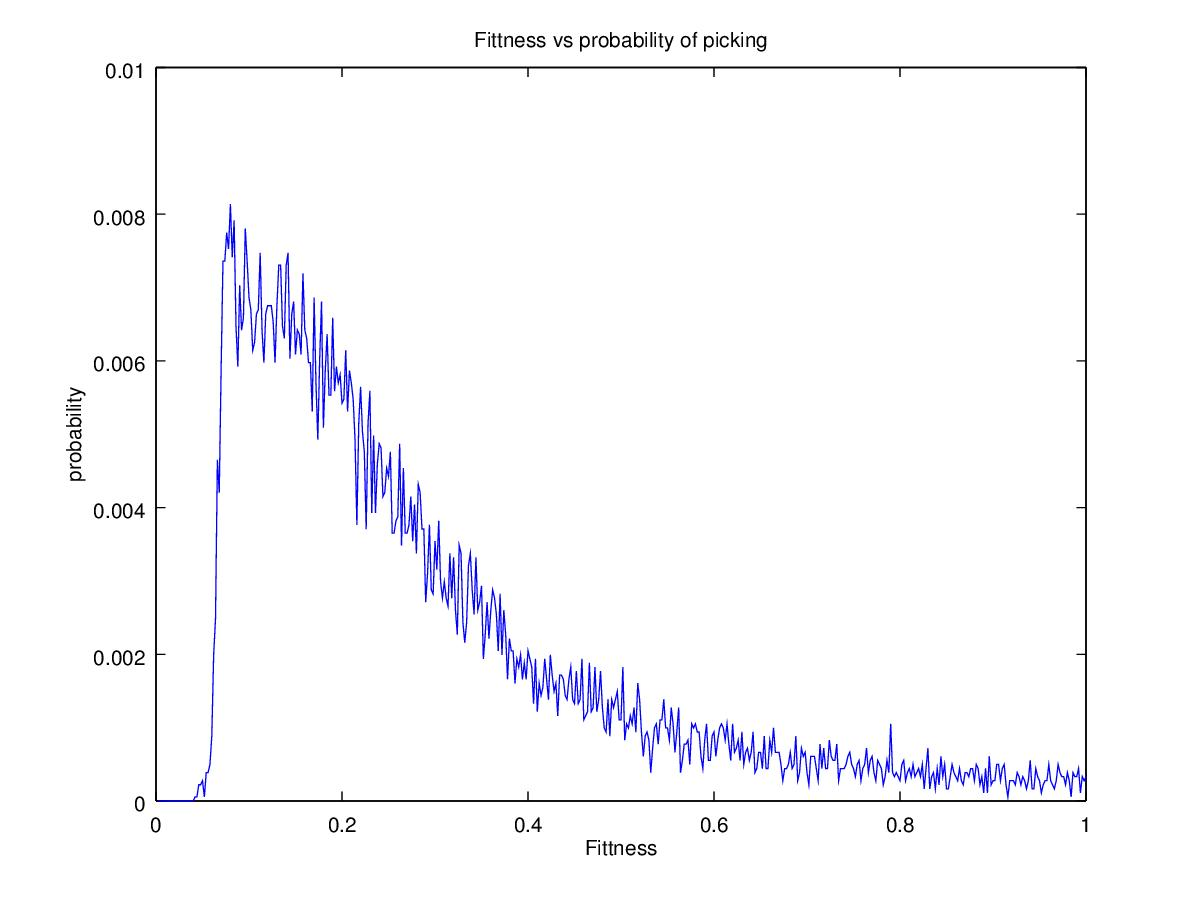
\includegraphics[width=60mm]{distrobution_1.jpg}
	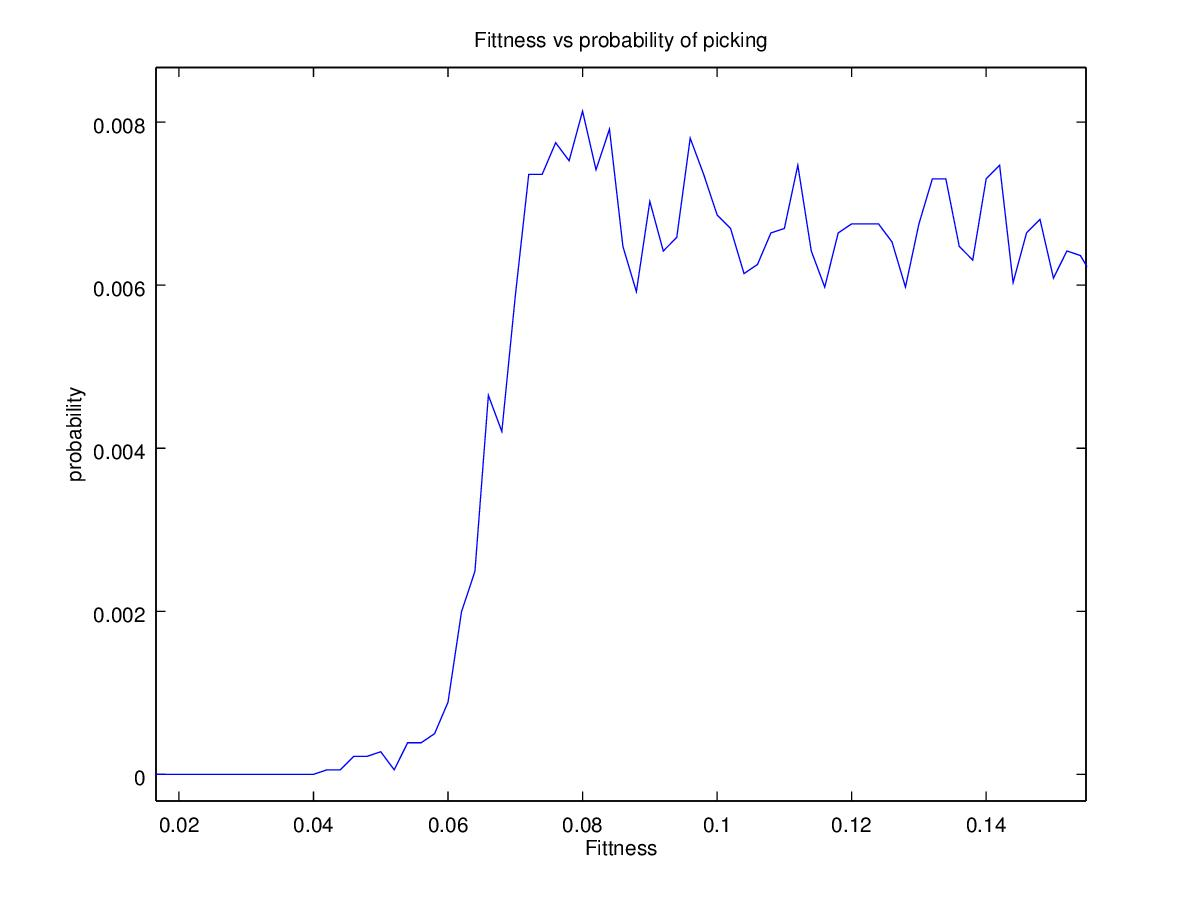
\includegraphics[width=60mm]{distrobution_2.jpg}
	\caption{Distribution of Optimization}
\end{figure}

This data gives us an idea of what the expected fitness would be of a randomly chosen greenhouse scheme. The mist and compressor control scheme for the Clarkson University Greenhouse were chosen based on intuition and not optimization. It is clear from the zoomed in graph that the vast majority of schemes are sub optimal. It is of our opinion that this is the most significant result discovered. It shows that there is huge potential for increasing the efficiency of Clarkson's Greenhouse watering system. A rough estimation is around half the compressor usage.

\subsection{Weaknesses}

We have seen that our model and optimization method achieve very good results and interesting data however there are several weaknesses.

\begin{itemize}
		  \item Assuming a linear drying rate is very wrong. Drying models are very complex and often impossible to solve analytically. Even the simplest models follow negative exponentials and require the geometries to be simple. I suspect that this weakness can only be overcome by measuring drying rates of real roots and interpolating the data. \cite{mujumdar2000fundamental}
		  \item The model is very sensitive to $\lambda_r$ and $\lambda_m$ and only by playing with these values can you determine meaningful schemes.
	     \item This is the biggest problem in the optimization. Optimal schemes vary radically. Running the optimization twice may produce to solutions that do equally well however the schemes will be completely different. Often times the top three schemes found are totally different.
\end{itemize}



\section{Future Work}

This project was developed under severe mountain dew limitations and would benefit greatly from more time. A major struggle was miss starts in different areas. It seemed very promising to solve this optimization probable analytically but it got to complex. We also wasted time trying to determine optimal control of mirrors that would shine light on the greenhouse. The biggest improvement we could make to our optimization is running more tests and implementing a better search algorithm. Originally the goal was to use simulated annealing to converge to the optimal scheme but this was never implemented. Currently a random search is used.  

\section{Discussion}
Our model seems to mimic the essential aspects of aeroponic water system. Using search algorithms we found optimal or sub optimal control scheme and related this problem to the Clarkson Greenhouse project. We have shown the importance of optimizing such a scheme and give evidence that a two fold decease in compressor usage can be achieved

\bibliography{mybib}{}
\bibliographystyle{plain}



\end{document}
